\section{Introduction}
\label{sec:intro}

\begin{figure}
    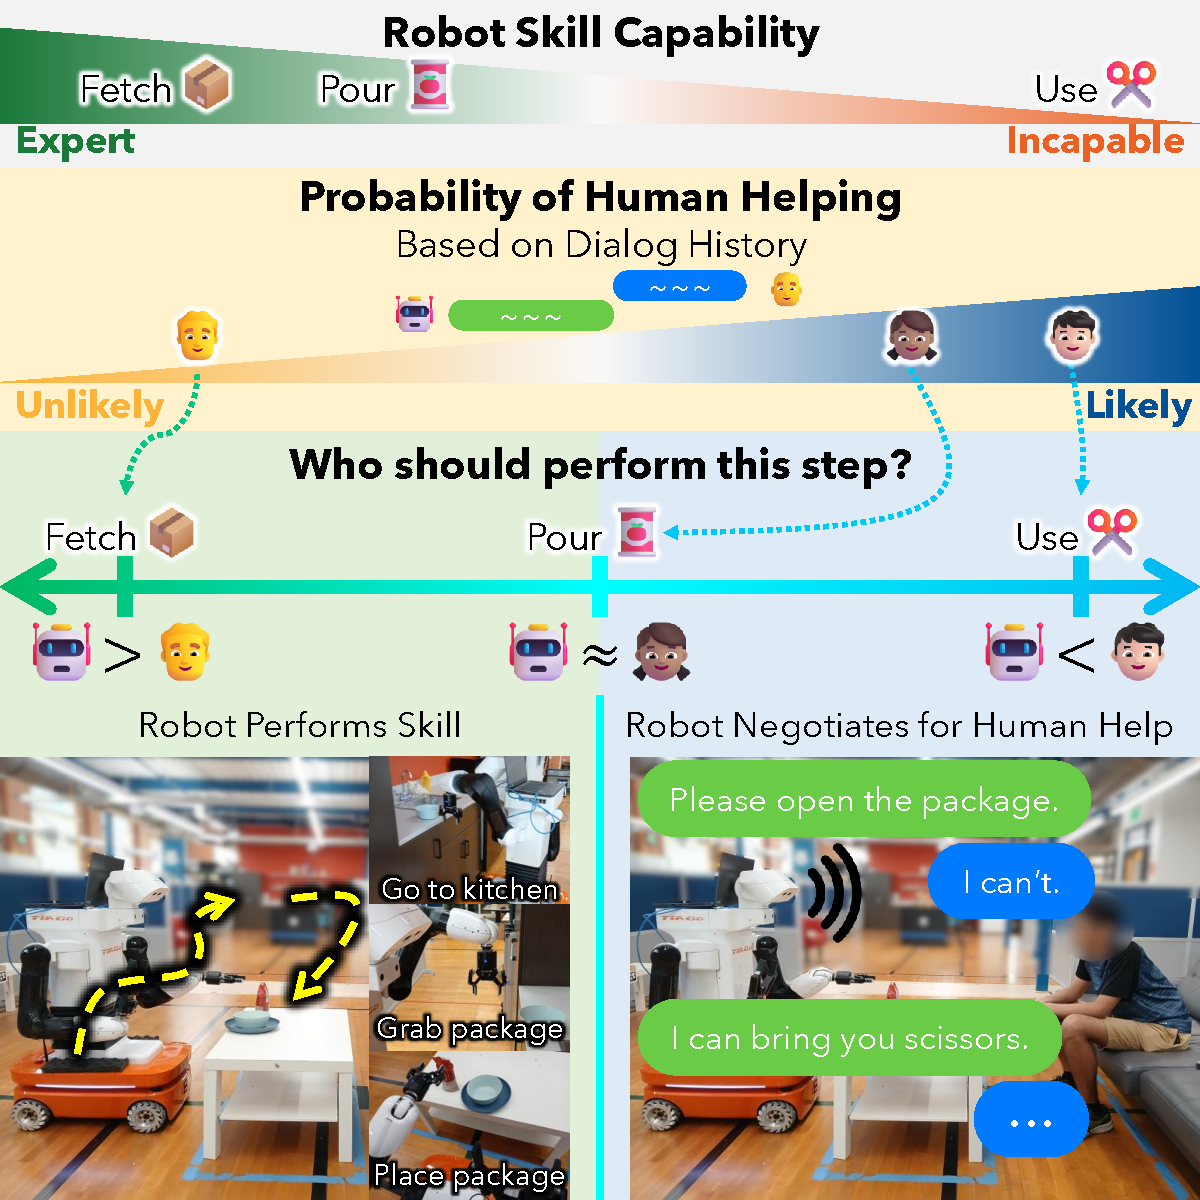
\includegraphics[width=1\columnwidth]{figs/fig1_option3_v5.pdf}
    \caption{We present \ours{}, a system for human-robot collaboration where both agents can initiate and carry out physical and verbal actions. \ours{} uses both the robot's capability and the likelihood of human helping (inferred from previous dialog history) to determine whether the robot is better suited than the human to perform the skill. If it is, it attempts the skill itself. If not, it negotiates for human help.}
    \label{fig:pull-fig}
\end{figure}


Imagine preparing for a dinner party with a friend. Your friend might excel at mixing drinks while you focus on cooking the main dish. You are also better at decorating, while both of you reluctantly negotiate over less desirable tasks like cleaning.

Now, imagine a helper robot in place of the friend. Current robots are not fully autonomous for many household tasks, but they offer broad capabilities with varying levels of reliability that can be leveraged through collaboration with humans. To be an effective partner, such a robot must communicate in physically grounded natural language, decide when to take initiative or defer to the human, negotiate task allocation based on strengths and preferences, and adapt to changing contexts. These ingredients are essential not only for collaborative household robots, but also for coding assistants, chatbots, and AI agents more broadly.


% Imagine working with your friend to prepare for a dinner party. Your friend might be an expert in creating punch while you prefer to cook the main dish. Similarly, your friend might be less aesthetically refined, so you are better suited to decorate the room. You both detest cleaning and must negotiate to split up undesirable tasks.

% Now imagine that instead of a friend, you have a helper robot to prepare for the party. In line with current technology, it is not fully autonomous on this task but has broad capabilities of varying success rates that you can harness by working with it. To be a good collaborator, the robot must communicate with you in physically-grounded natural language, discern when to proactively step up or relinquish control to you, discuss with you to decide who is best suited to perform which subtasks, and adapt to your changing availability and preferences.
% These are key ingredients of not just good collaborative household robots, but also collaborative coding agents, chatbots, and AI agents in general.

% Achieving full autonomy on complex physical tasks in unstructured environments is an ultimate goal in robotics, yet it remains largely hindered by the limited, current capabilities of robots. Absent full autonomy, the utility of robots can still be tapped through close collaboration with humans.
% Such collaboration requires robots to communicate in natural language grounded in the physical world, discern when to proactively step up or relinquish control to the human collaborator, and engage in back-and-forth discussion to decide which agent is best suited to perform each part of a task.
% These are key ingredients of not just good collaborative household robots, but also collaborative coding agents, chatbots, and AI agents in general.

Long-horizon tasks, such as preparing for a party, require dynamic, bidirectional collaboration across control, initiative, and communication. In particular, the ability to both take initiative and yield control is central to effective human–AI teamwork. However, current AI systems (e.g., chatbots) typically rely on one-directional, human-initiated interactions~\cite{ouyang2022training, achiam2023gpt}, while prior human–robot interaction (HRI) approaches often assume fixed collaboration plans and full human compliance~\cite{selvaggio2021autonomy}. Such assumptions limit flexibility and fail to account for the diverse preferences, capabilities, and strengths of different human partners. We argue that effective human–robot collaboration requires a paradigm shift toward mixed-initiative dialog as the communicative medium, enabling both agents to initiate, negotiate, and respond to proposals in natural language.

% Long-horizon robotics tasks like preparing for a party necessitate dynamic collaboration, which is inherently bidirectional---in control, initiative, and communication.
% Taking initiative and yielding control is particularly important in Human-AI collaboration, but current AI systems (e.g., chatbots) are driven by single-directional, human-initiated interactions~\cite{ouyang2022training, achiam2023gpt}, while prior human-robot interaction (HRI) solutions often assume full control over the collaboration plan and full human co-operation~\cite{selvaggio2021autonomy}.
% Such systems are inflexible, unable to adapt to the wide distribution of human collaborators and their preferences, capabilities, and strengths.
% We argue that to elicit the complementary strengths of both agents, effective human-robot collaboration demands a paradigm shift toward using mixed-initiative dialog as a communicative medium, in which \textit{both} agents can initiate, negotiate, and respond to proposals using natural language.

\begin{figure*}[htbp]
    \centering
    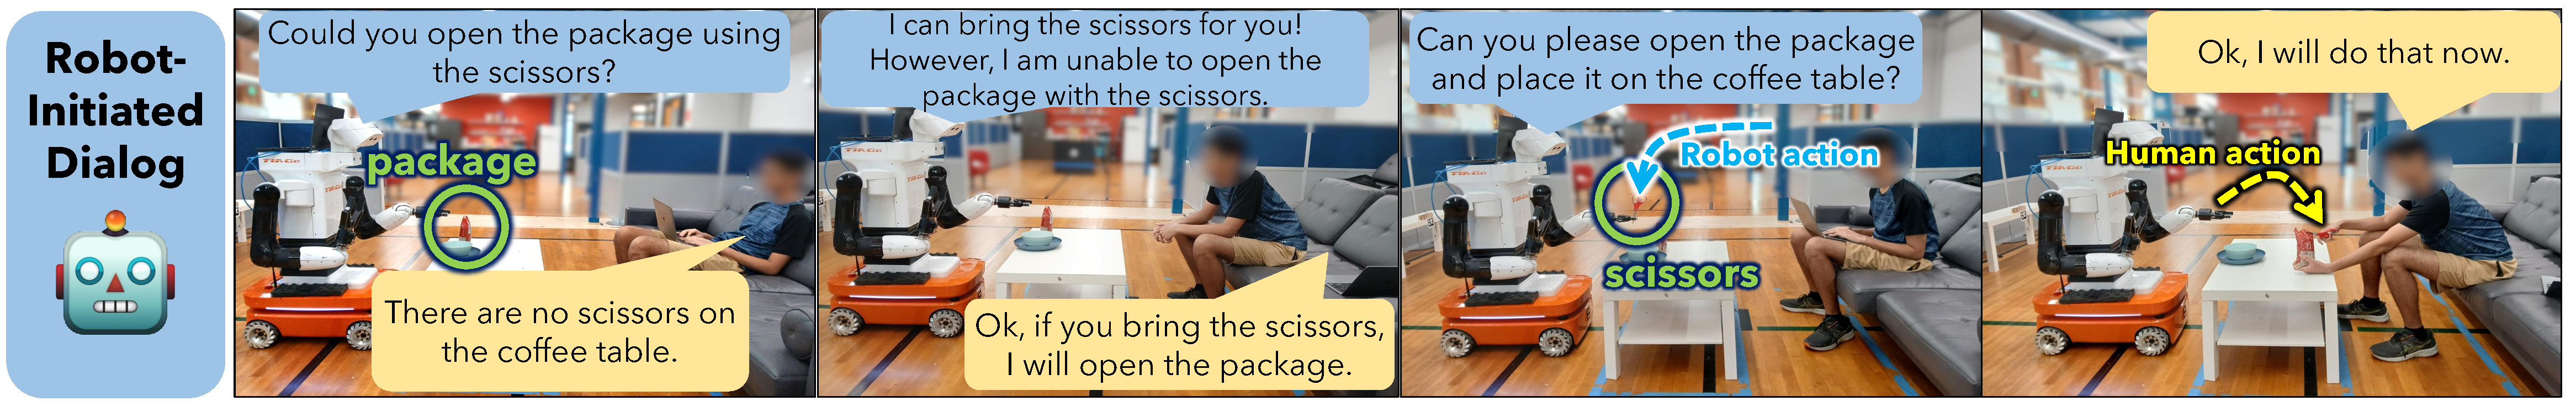
\includegraphics[width=1\textwidth]{figs/fig1_robot_init_v2.pdf}
    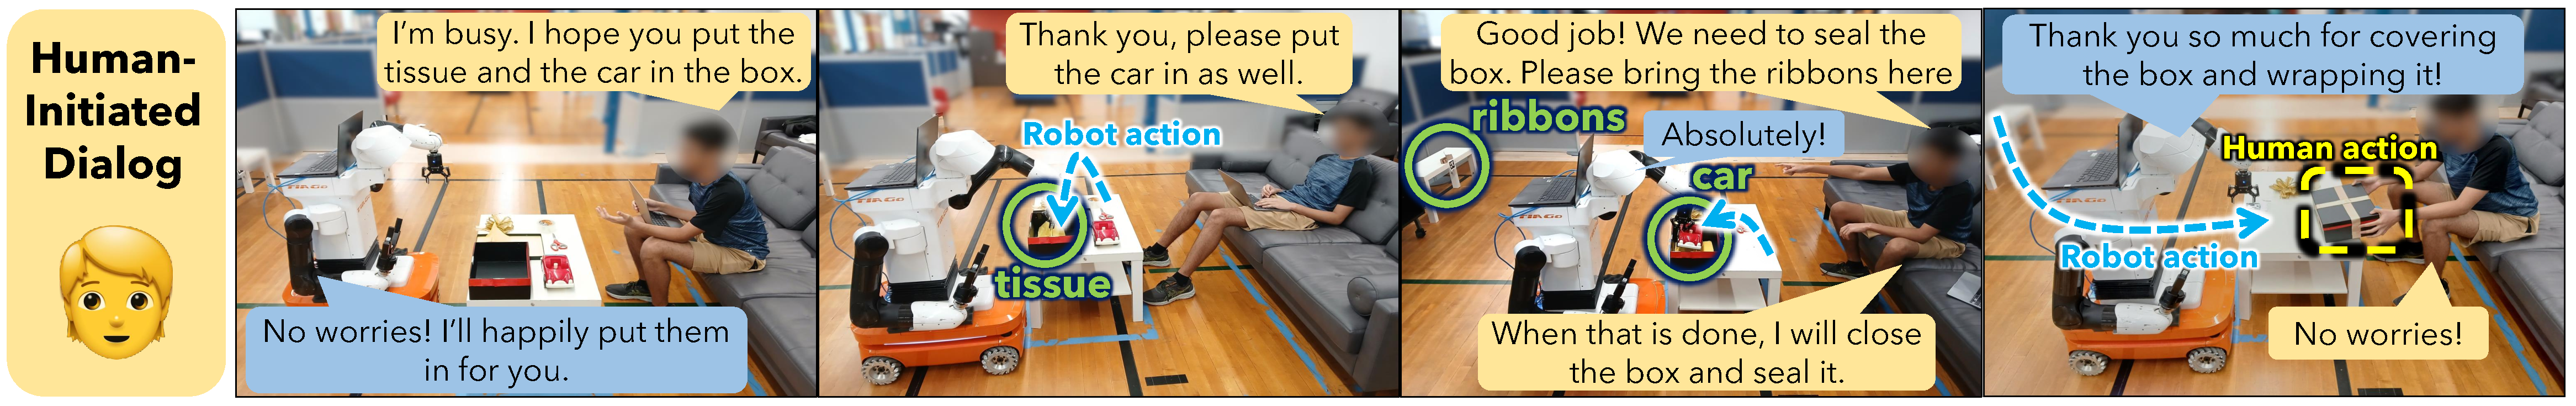
\includegraphics[width=1\textwidth]{figs/fig1_human_init_v2.pdf}
    \caption{\ours{} supports \textit{both} robot-initiated (top row) \textit{and} human-initiated (bottom row) task-directed speech2speech dialog, where both agents discuss who is best suited to perform steps in a long-horizon task. These are real dialog and physical interactions from our user studies (see our
    % \href{mico-bot.github.io}{website}
    website\textsuperscript{1}).}
    \label{fig:teaser}
    \vspace{-5mm}
\end{figure*}

To enable this paradigm shift, we introduce \ours{} (Mixed-Initiative Collaborative roBot), the first system that supports mixed-initiative dialog for seamless human–robot collaboration in the physical world. \ours{} allocates task steps to the most suitable agent (see Fig. ~\ref{fig:pull-fig}) in a way that maximizes overall success, minimizes human effort, and respects human-initiated requests. It achieves this by engaging in mixed-initiative dialog and negotiation to decide step allocation (see Fig.~\ref{fig:teaser}), while coordinating the physical and verbal actions required to execute the plan.

% To facilitate this paradigm shift, we introduce \ours{} (Mixed-Initiative Collaborative roBot), the first system to enable mixed-initiative dialog toward more seamless human-robot collaboration in the physical world.
% \ours{} aims to find the most suitable agent to perform each step of the task in an allocation that maximizes success, minimizes human effort, and respects any human-initiated requests. It does so by engaging in mixed-initiative dialog and negotiation with a human on how to allocate task steps, coordinating the physical and verbal actions needed to execute the plan.

To realize this objective across diverse humans and long-horizon tasks, \ours{} optimizes decision-making at three levels. First, a meta-planner determines the high-level collaboration strategy, integrates human-specified preferences, and generates adaptive code for robot actions (verbal or physical). Second, a planner executes this code, selecting the optimal collaboration approach based on the environment state, a simulation-trained affordance model of robot capabilities, and a dynamic estimate of human helpfulness derived from prior interactions. Finally, an action executor carries out the next step of the plan, whether it involves manipulation, dialog initiation, or dialog response.

% To collaborate under this objective on a wide range of humans on long-horizon tasks, \ours{} makes optimization decisions across three levels. First, a meta-planner determines the high-level collaborative strategy, incorporating human-specified preferences and creating adaptive code to generate robot actions (verbal or physical). Second, a planner executes the generated code to determine the optimal collaboration approach given the current environment state, the robot's capabilities via a simulation-trained affordance model, and a dynamic evaluation of the human's helpfulness based on prior interactions. Finally, an action executor carries out the next step of the plan---either a manipulation action, dialog initiation, or response to human dialog.

We validate \ours{} through extensive evaluation in both simulation and the real world. In simulation, we test against LLM-simulated humans with varying helpfulness and responsiveness; in real-world experiments, 18 participants collaborated with a TIAGo mobile manipulator on three household tasks. Our approach improves success rate by \textbf{50\%} compared to a pure LLM baseline and is preferred by over \textbf{75\%} of participants.

% Through extensive experimental evaluation, we thoroughly validate our system in both simulation (with LLM-simulated humans of varying helpfulness and responsive moods) and the real-world through a user study involving 18 unique participants collaborating with a Tiago mobile manipulator on three household tasks.
% Our approach outperforms a pure LLM baseline by \textbf{50\%} in success rate and was preferred by over \textbf{70\%} of participants.

In summary, our contributions are:

\begin{itemize}

\item \textbf{A new problem setting} that integrates mixed-initiative natural language dialog with mixed-initiative human–robot interaction.

\item \textbf{A novel optimization framework} for task allocation that balances human and robot effort with success through a unified metric.

\item \textbf{A collaborative simulation environment} built on MiniBehavior~\cite{jin2023minibehavior}, featuring LLM-controlled virtual humans, with an interactive demo on our project site.\footnotemark[1]

\item \textbf{A hierarchical robotic system, \ours{}}, that enables mixed-initiative speech-to-speech human–robot collaboration and flexibly adapts to diverse real human collaborators in physically grounded, long-horizon tasks.

\end{itemize}
% In summary, our work's contributions are four-fold: (1) we introduce a \textbf{new problem setting} that integrates mixed-initiative natural language dialog with mixed-initiative human-robot interaction; (2) we propose a novel \textbf{optimization framework} for task allocation, balancing human and robot effort and success through a unified metric; (3) we provide a \textbf{new simulator} for collaborative household tasks built on top of MiniBehavior~\cite{jin2023minibehavior} that includes LLM-controlled virtual humans and is available on our project site;\footnotemark[1]
% % \href{https://mico-bot.github.io}{our website}
% and (4) we develop a \textbf{robotic system and framework}, \ours{}, a three-level hierarchical solution for mixed-initiative speech2speech human-robot collaboration that flexibly adapts to a wide range of real human collaborators in physically grounded, long-horizon tasks.